\documentclass[letterpaper, 11pt]{article}

% set version variable
\newcommand{\versionnumber}{0.1}

% russian language
\usepackage[utf8]{inputenc}
\usepackage[T2A]{fontenc}
\usepackage[english, russian]{babel}

% math
\usepackage{mathtools}
\usepackage{amsmath}

\usepackage{amssymb} % some math symbols
% abs function
\DeclarePairedDelimiter{\abs}{\lvert}{\rvert}

% enumerate
\usepackage{enumerate}

% set type and margins of the page
\usepackage{geometry}  % document margins
\geometry{letterpaper, left=1.4in, right = 1.4in, top = 1.7in, bottom = 1.7in}

% color links in content
\usepackage{hyperref}
\hypersetup{
    colorlinks=true,
    linkcolor=red,
    urlcolor=blue,
    linktoc=all
}

% indent at first \par after section
\usepackage{indentfirst}

% fixed table and figures in section
\usepackage{float}

% colors
\usepackage{color}
\usepackage[usenames,dvipsnames]{xcolor}

% paragraph indent
\setlength{\parskip}{0.5em}

% pseudocode
\usepackage{algorithmicx}
\usepackage{algpseudocode}

\title{\large{Краткий конспект}\\
\LARGE{Лекция 4. Суффиксные деревья}\\
\normalsize версия \versionnumber (\textcolor{NavyBlue}{draft})}
\date{7 марта, 2016}
\author{\underline{Д. Ищенко\thanks{МФТИ}} \and Б. Коварский\footnotemark[1]
\and И. Алтухов\footnotemark[1] \and Д. Алексеев\footnotemark[1]}

\begin{document}
\maketitle
\thispagestyle{empty}
\clearpage

% let's go
\section{Задача поиска k мотивов в геноме}

Вернемся к задаче поиска мотива $m$ в геноме $g$. В лекции о Z-алгоритме мы выяснили, что ее можно решить за линейное время $O(|m| + |g|)$, где $|m|$ - длина мотива, $|g|$ - длина генома. Представим, что необходимо найти $k$ различных мотивов в геноме $g$. Используя предыдущий метод, мы будем конструировать <<Z-ящики>> для каждой объединенной строки $m\$g$ и производить поиск. Соответственно временная сложность алгоритма вырастет до $O(k(|m| + |g|))$, в виду того, что $|m| << |g|$, сложность - $O(k|g|)$.

В реальных задачах $k$ может иметь достаточно большое значение, например, при картировании ридов (коротких прочтений) на референсный геном, значения $k$ могут быть порядка $10^6 - 10^8$. Возникает необходимость оптимизации алгоритма. В этой лекции мы рассмотрим такую конструкцию, как суффиксное дерево и покажем, как с помощью него решить задачу поиска мотива и несколько других задач, существенно уменьшив временную сложность вычислений относительно Z-алгоритма.

\section{Cуффиксное дерево}

По аналогии с ранее введенными префиксами строки $S$ длиной $n$, назовем \textbf{$k$-ым суффиксом} строки $S$ ее подстроку, начинающуюся с $k$-го и заканчивающуюся последним символом: $S[k..n]$. Например, для строки ATGCAT все множетсво суффиксов будет представлять из себя:
\begin{verbatim}
1: ATGCAT
2: TGCAT
3: GCAT
4: CAT
5: AT
6: T
\end{verbatim}

Отметим, что количество всех суффиксов строки $S$ равно ее длине, а также тот факт, что полная строка также является суффиксом самой себя (первый суффикс).

Введем понятие \textit{суффиксного дерева}. В общем виде -- это древовидный граф с набором вершин и ребер, создающийся из всех суффиксов последовательности $S$. В графе к каждому ребру приписана <<метка>>, соответствующая некоторой подстроке из $S$. Двигаясь по ребрам от выделенной вершины суффиксного дерева, называемой корнем, к одному из листьев дерева (вершине, к которой ведет только одно ребро) и соединяя последовально <<метки>> ребер в одну последовательность, в конечном итоге мы получаем один из суффиксов исходной последовательности $S$. Неформально процесс создания суффиксного дерева можно описать следующим образом:
\begin{enumerate}[(i)]
\item
допишем в конец последовательности $S$ символ, не встречающийся в самой последовательности, например: \textbf{\$}, тем самым получим последовательность $S^{*} = S\$$
\item
возьмем все суффиксы последовательности $S^{*}$, <<закрепим>> их начала в одной вершине, называемой корнем дерева (Рис. 1), в <<концы>> суффиксов поместим вершины и соединим их ребрами с корнем дерева. Вершины пронумеруем от $1$ до $n$. Припишем к ребрам <<метки>> равные соответствующим суффиксам.
\item
<<склеим>> совпадающие начала ребер. Образованный граф представляет из себя суффиксное дерево для исходной последовательности S.
\end{enumerate}

\begin{figure}[H]
  \center{
  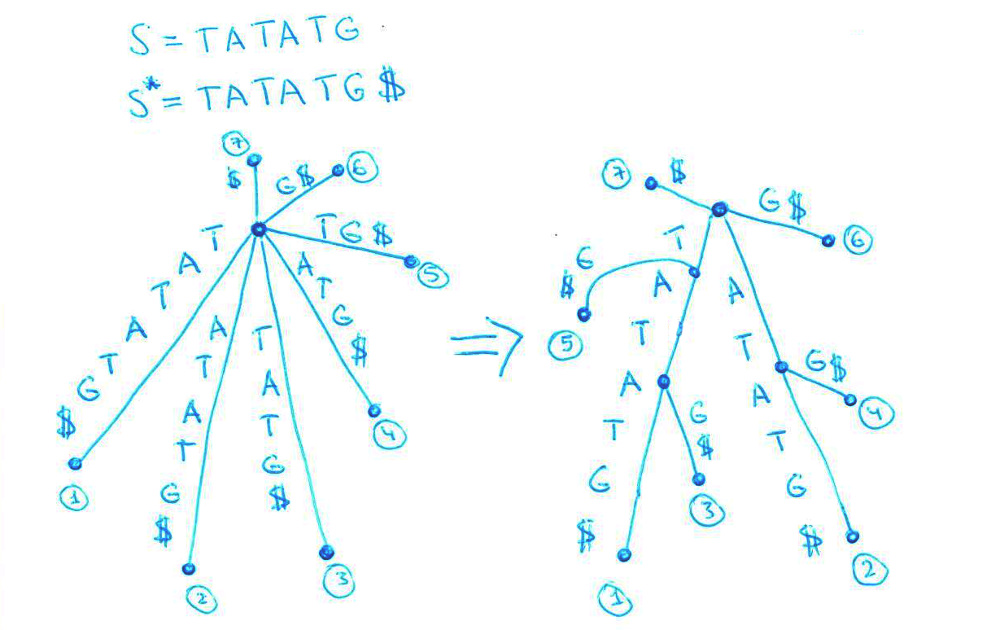
\includegraphics[scale = 0.85]{fig/fig1.jpg}
  }
  \caption{Создание суффиксного дерева для последовательности $S$.}
\end{figure}

\clearpage
Перечислим несколько свойств суффиксного дерева:
\begin{enumerate}[(i)]
\item
Количество листьев дерева равно количеству суффиксов последовательности $S^*$.
\item
Каждый узел в дереве, кроме корневого, имеет ровно один родительский узел.
\item
Двигаясь по ребрам от корня дерева к одному из \textit{листьев} и объединяя метки соответствующих ребер в одну последовательность, последняя будет соответствовать одному из \textit{суффиксов} последовательности $S^*$.
\item
Двигаясь по ребрам от корня дерева к одной из \textit{внутренних вершин} дерева и объединяя метки соответствующих ребер в одну последовательность, последняя будет соответствовать некоторой \textit{подстроке} из $S^*$.
\item
Для любой подстроки $S^*$ можно найти соответсвующий ей путь от корня дерева к одной из вершин.
\item
Метки ребер выходящих из корня или любой внутренней вершины отличаются первыми символами (иначе они были бы склеены в одно ребро). Следовательно из любой вершины не может выходить больше $\sigma + 1$ ребер, где $\sigma$ -- размер алфавита (количество разных символов, для нуклеотидной последовательности $\sigma = 4$).
\item
Если общее число вершин в дереве равно $N$, то число ребер: $(N - 1)$.

Предположим, что мы построили для последовательности $S$ суффиксное дерево, как с помощью него определить количество вхождений мотива $p$ в строку $S$?
\end{enumerate}

\clearpage
\section{Алгоритм посроения $O(n^2)$}
\par


\begin{algorithmic}[1]
\Procedure{TreeCreation}{$S$}
\State $S = S + " \$ "$
\State $nodes \gets [[1], [-1]]$
\State $edges \gets [, S]$

\item[]
\For{$i\gets 1, len(S)$}
\State $suf \gets S[i..len(S)]$
\State $j \gets 0$
\State $cur\_node \gets 0$
\State $to\_node \gets -1$
\State $isAdded \gets False$

\item[]
\While{not isAdded}
\For{$k \;\; in \;\;  nodes[cur\_node]$}
\If{$suf[j] = edges[k][0]$}
\State $to\_node \gets k$
\EndIf
\EndFor

\item[]

\If{$to\_node = -1$}
\State $...$ \Comment{Добавляем новый лист и ребро}
\State $isAdded \gets True$
\Else
\For{$p \gets 1, len(edges[to\_node])$}

\If{$suf[j + p] != edges[to\_node][p]$}
\State $...$ \Comment{Добавляем новый лист и внутреннюю вершину}
\State $isAdded \gets True$
\State $break$
\EndIf

\EndFor

\State $j \gets j + len(edges[to\_node])$
\State $cur\_node = to\_node$

\EndIf

\EndWhile

\EndFor
\item[]
\State \Return $[nodes, edges]$
\EndProcedure
\end{algorithmic}


\clearpage
\section{Поиск в глубину}
\par
Решаем задачу поиска мотива, как посчитать количество вхождений?

\begin{algorithmic}[1]
\Procedure{LeavesCount}{$i$, $nodes$}
\If{$nodes[i][0] = -1$}
\State \Return $1$
\EndIf
\item[]
\State $lCount \gets 0$
\For{$k \;\; in \;\; nodes[i]$}
\State $lCount = lCount + LeavesCount(k, nodes)$
\EndFor
\item[]
\State \Return $lCount$
\EndProcedure
\end{algorithmic}

\section{Какие еще задачи можно решить с помощью дерева}
\par
Поиск повтора, поиск максимальной общей подстроки, нечеткий поиск.

\section{Ссылки}

\begingroup
\renewcommand{\section}[2]{}%
\begin{thebibliography}{7}


\end{thebibliography}
\endgroup

\end{document}
